\section{Appendix}

\createsectiontoc{}

\subsection{Trigonometry}
\subsubsection{Common angles}
\begin{center}
    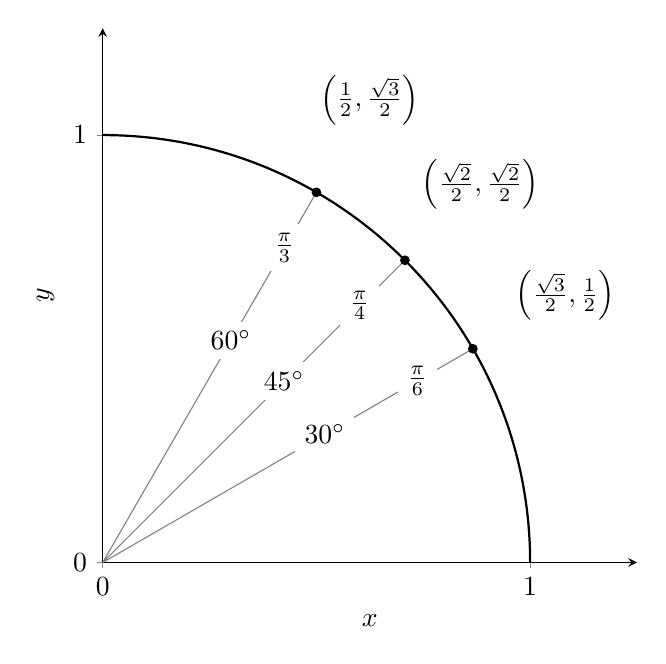
\begin{tikzpicture}
        \begin{axis}[
                width=0.8\linewidth,
                unit vector ratio={1 1},
                axis x line=left,
                axis y line=left,
                xmin=0,
                xmax=1.25,
                ymin=0,
                ymax=1.25,
                xlabel={$x$},
                ylabel={$y$},
                xtick={0, 1},
                ytick={0, 1},
                mark=none,
            ]
            \draw[thick] (0,0) circle(1);

            \draw[gray] \foreach \i in {30,45,60} {(0,0) -- ({cos(\i)},{sin(\i)})};
            \filldraw[black] \foreach \i in {30,45,60} {(\i:1) circle(0.01)};
            \draw \foreach \i in {30,45,60} {(\i:0.6) node[fill=white] {$\i^\circ$}};
            \draw \foreach \i/\itext in {30/\frac{\pi}{6},45/\frac{\pi}{4},60/\frac{\pi}{3}} {(\i:0.85) node[fill=white] {$\itext$}};

            \draw \foreach \i/\itext/\y in {
                    30/\frac{\sqrt{3}}{2}/\frac{1}{2},
                    45/\frac{\sqrt{2}}{2}/\frac{\sqrt{2}}{2},
                    60/\frac{1}{2}/\frac{\sqrt{3}}{2}} {(\i:1.25) node[fill=white] {$\left(\itext,\y\right)$}};
        \end{axis}
    \end{tikzpicture}
\end{center}

\subsubsection{Identities}
Given: $n, j \in \mathbb{N}$
\begin{align*}
     & \sin(\pi n)                                                                                 & = & \: 0                                                       \\
     & \cos(\pi n)                                                                                 & = & \: {(-1)}^n                                                \\
     & \sin\left(\frac{\pi}{2}n\right) = \left(\frac{1 + {(-1)}^n}{2}\right){(-1)}^{\frac{n+2}{2}} & = & \begin{cases} 0 &n=2j \\ {(-1)}^j&n=2j+1 \end{cases}       \\
     & \sin\left(\frac{3\pi}{2}n\right)                                                            & = & \begin{cases} 0 &n=2j \\ {(-1)}^{j+1}&n:\, odd \end{cases} \\
     & \cos\left(\frac{\pi}{2}n\right) = \left(\frac{1+{(-1)}^n}{2}\right){(-1)}^{\frac{n}{2}}     & = & \begin{cases} {(-1)}^j &n=2j \\ 0 &n=2j+1 \end{cases}      \\
     & \cos\left(\frac{3\pi}{2}n\right)                                                            & = & \begin{cases} {(-1)}^{j} &n=2j \\ 0 &n=2j+1 \end{cases}    \\
     & \sin\left(\left(n\pm 1\right)\frac{\pi}{2}\right)                                           & = & \pm \cos\left(\frac{n\pi}{2}\right)                        \\
     & \cos\left(\left(n\pm 1\right)\frac{\pi}{2}\right)                                           & = & \mp \sin\left(\frac{n\pi}{2}\right)                        \\
     & \sin(90^\circ\pm\alpha) = \sin(\frac{\pi}{2} \pm \alpha)                                    & = & \cos(\alpha)                                               \\
     & \cos(90^\circ\pm\alpha) = \cos(\frac{\pi}{2} \pm \alpha)                                    & = & \mp\sin(\alpha)                                            \\
     & \sin(180^\circ\pm\alpha) = \sin(\pi \pm \alpha)                                             & = & \mp\sin(\alpha)                                            \\
     & \cos(180^\circ\pm\alpha) = \cos(\pi \pm \alpha)                                             & = & -\cos(\alpha)                                              \\
     & \frac{1}{\sin^2 \alpha}                                                                     & = & 1+\cot^2 (\alpha)                                          \\
     & \frac{1}{\cos^2 \alpha}                                                                     & = & 1+\tan^2 (\alpha)                                          \\
     & {(-1)}^n+{(-1)}^{-n}=e^{in\pi}+e^{-in\pi}                                                   & = & 2\cos(\pi n)                                               \\
     & {(-1)}^n-{(-1)}^{-n}=e^{in\pi}-e^{-in\pi}                                                   & = & 2i\sin(\pi n)
\end{align*}

\subsubsection{Goniometry}
\noindent
\begin{align*}
    \sin(x\pm y) & =\sin(x)\cos(y)\pm\cos(x)\sin(y)              \\
    \cos(x\pm y) & =\cos(x)\cos(y)\mp\sin(x)\sin(y)              \\
    \tan(x\pm y) & =\frac{\tan(x)\pm\tan(y)}{1\mp\tan(x)\tan(y)}
\end{align*}
\begin{align*}
    \sin(2x)                     & =2\sin(x)\cos(x)                         \\
    \cos(2x)=\cos^2(x)-\sin^2(x) & =1-2\sin^2(x)=2\cos^2(x)-1               \\
    \tan(2x)                     & =\frac{2\tan(x)}{1-\tan^2(x)}            \\
    \sin(3x)                     & =3\sin(x)-4\sin^3(x)                     \\
    \cos(3x)                     & =4\cos^3(x)-3\cos(x)                     \\
    \tan(3x)                     & =\frac{3\tan(x)-\tan^3(x)}{1-3\tan^2(x)}
\end{align*}
\begin{align*}
    \sin^2\left(\frac x2\right)    & =\frac{1-\cos(x)}{2}                                 \\
    \cos^2\left(\frac x2\right)    & =\frac{1+\cos(x)}{2}                                 \\
    \tan^2\left(\frac{x}{2}\right) & =\frac{1-\cos(x)}{1+\cos(x)}                         \\
    \tan\left(\frac x2\right)      & =\frac{1-\cos(x)}{\sin(x)}=\frac{\sin(x)}{1+\cos(x)}
\end{align*}
\begin{align*}
    \sin(x)\cos(y)      & =\frac12\Bigl[\sin(x+y)\;+\;\sin(x-y)\Bigr] \\
    \sin(x)\sin(y)      & =\frac12\Bigl[\cos(x-y)\;-\;\cos(x+y)\Bigr] \\
    \cos(x)\cos(y)      & =\frac12\Bigl[\cos(x+y)\;+\;\cos(x-y)\Bigr] \\
    \sin(x)\pm\sin(y)   & =2\sin\frac{x\pm y}{2}\cos\frac{x \mp y}{2} \\
    \cos(x)+\cos(y)     & =2\cos\frac{x+y}{2}\cos\frac{x-y}{2}        \\
    \cos(x)-\cos(y)     & =-2\sin\frac{x+y}{2}\sin\frac{x-y}{2}       \\
    \tan(x) \pm \tan(y) & = \frac{\sin(x\pm y)}{\cos(x)\cos(y)}
\end{align*}

\subsubsection{Transformations}

\renewcommand{\arraystretch}{1.3}

\setlength\tabcolsep{6pt} % default value: 6pt

\begin{tabularx}{\linewidth}{@{}p{0.15\linewidth}ccc@{}}
                                                    & $\sin$                                         & $\cos$                                         & $\tan$                                         \\
    \cmidrule{2-4}
    $\sin(\alpha)=$                                 &                                                & $\sqrt{1-\cos^2(\alpha)}$                      & $\frac{\tan(\alpha)}{\sqrt{1+\tan^2(\alpha)}}$ \\
    $\cos(\alpha)=$                                 & $\sqrt{1-\sin^2(\alpha)}$                      &                                                & $\frac{1}{\sqrt{1+\tan^2(\alpha)}}$            \\
    $\tan(\alpha)=$ \newline $\alpha \neq 90^\circ$ & $\frac{\sin(\alpha)}{\sqrt{1-\sin^2(\alpha)}}$ & $\frac{\sqrt{1-\cos^2(\alpha)}}{\cos(\alpha)}$ &
\end{tabularx}

\renewcommand{\arraystretch}{1}

\setlength\tabcolsep{6pt} % default value: 6pt

\subsubsection{Euler-Relation}
\noindent
\begin{align*}
    \sin(x)    & =\frac{1}{2i}(e^{ix}-e^{-ix})             \\
    \cos(x)    & =\frac{1}{2}(e^{ix}+e^{-ix})              \\
    \tan(x)    & =\frac{e^{ix}-e^{-ix}}{i(e^{ix}+e^{-ix})} \\
    \sinh(x)   & =\frac{1}{2}(e^{x}-e^{-x})                \\
    \cosh(x)   & =\frac{1}{2}(e^{x}+e^{-x})                \\
    \tanh(x)   & =\frac{e^{x}-e^{-x}}{(e^{x}+e^{-x})}      \\
    e^{ix}     & = \cos(x) + i \cdot \sin(x)               \\
    e^{k\pi i} & = \begin{cases}
                       1  & k = 2n     \\
                       -1 & k = 2n + 1
                   \end{cases} \quad n \in \mathbb{N}
\end{align*}

\subsubsection{Inverse functions}
\noindent
\begin{align*}
    \sin(\arccos(x))                         & = \sqrt{1-x^2}                                                 \\
    \cos(\arcsin(x))                         & =\sqrt{1-x^2}                                                  \\
    \sin(\arctan(x))                         & =\frac{x}{\sqrt{x^2+1}}                                        \\
    \cos(\arctan(x))                         & =\frac{1}{\sqrt{x^2+1}}                                        \\
    \tan(\arcsin(x))                         & =x \cdot {(1-x)}^{-\frac{1}{4}}                                \\
    \tan(\arccos(x))                         & =x^{-1} \cdot {(1-x)}^{\frac{1}{4}}                            \\
    \operatorname{arcsinh}(x)                & =\ln(x+\sqrt{x^2+1})                                           \\
    \operatorname{arccosh}(x)                & =\ln(x+\sqrt{x^2-1})                                           \\
    \operatorname{arctanh}(x)                & =\frac{1}{2}\cdot \ln(\frac{1+x}{1-x}); \quad \vert x\vert < 1 \\
    \operatorname{arccoth}(x)                & =\frac{1}{2}\cdot \ln(\frac{1+x}{x-1}); \quad \vert x\vert > 1 \\
    \sinh(2 \cdot \operatorname{arcsinh}(x)) & =2x\sqrt{x^2-1}                                                \\
    \sinh(\operatorname{arccosh}(x))         & =\sqrt{x^2-1};\qquad x>0                                       \\
    \cosh(\operatorname{arcsinh}(x))         & =\sqrt{x^2+1}
\end{align*}

\subsection{Derivatives}

\textbf{Sums and Constants}
\begin{align*}
    (f\pm g)'             & =f'\pm g'                                  \\
    {(c\cdot f)}^{\prime} & =c\cdot f^{\prime}\quad(c\text{ constant})
\end{align*}

\textbf{Product/ Quotient Rule}
\begin{align*}
    (f\cdot g)'                      & =f'\cdot g+f\cdot g'                             \\
    {\left(\frac fg\right)}^{\prime} & =\frac{f^{\prime}\cdot g-f\cdot g^{\prime}}{g^2}
\end{align*}

\textbf{Reciprocal Rule}
\begin{align*}
    {\left(\frac{1}{f}\right)}^{\prime} & = -\frac{f^{\prime}}{f^2}
\end{align*}

\textbf{Chain Rule}
\begin{align*}
    {[f(g(x))]}^{\prime}          & =f^{\prime}(g(x))\cdot g^{\prime}(x)                         \\
    F'(t)                         & =f_x(x(t),y(t))\cdot\dot{x}(t)+f_y(x(t),y(t))\cdot\dot{y}(t) \\
    \frac{\partial y}{\partial x} & = \frac{\partial y}{\partial u}\frac{\partial u}{\partial x}
\end{align*}

\subsubsection{Common Derivatives}
\noindent
\begin{align*}
     & \frac{d}{dx}x^n                       &  & =nx^{n-1}                              \\
     & \frac{d}{dx}e^x                       &  & =e^x                                   \\
     & \frac{d}{dx}a^x                       &  & =a^x\ln(a),\quad a>0                   \\
     & \frac{d}{dx}\ln(x)                    &  & =\frac1x                               \\
     & \frac{d}{dx}\log_a(x)                 &  & =\frac1{x\ln(a)}                       \\
     & \frac{d}{dx}\sin(x)                   &  & =\cos(x)                               \\
     & \frac{d}{dx}\cos(x)                   &  & =-\sin(x)                              \\
     & \frac{d}{dx}\tan(x)                   &  & =\frac1{\cos^2(x)}=1+\tan^2(x)         \\
     & \frac{d}{dx}\arcsin(x)                &  & =\frac1{\sqrt{1-x^2}}                  \\
     & \frac{d}{dx}\arccos(x)                &  & =-\frac1{\sqrt{1-x^2}}                 \\
     & \frac{d}{dx}\arctan(x)                &  & =\frac1{1+x^2}                         \\
     & \frac{d}{dx}\sinh(x)                  &  & =\cosh(x)                              \\
     & \frac{d}{dx}\cosh(x)                  &  & =\sinh(x)                              \\
     & \frac{d}{dx}\tanh(x)                  &  & =\frac{1}{\cosh^{2}(x)}=1-\tanh^{2}(x) \\
     & \frac{d}{dx}\sinh(x)                  &  & =\frac1{\sqrt{x^2+1}}                  \\
     & \frac{d}{dx}\operatorname{arccosh}(x) &  & =\frac1{\sqrt{x^2-1}}                  \\
     & \frac{d}{dx}\operatorname{arctanh}(x) &  & =\frac1{1-x^2}
\end{align*}

\subsection{Integral calculus}
\textbf{Hauptsatz}
\begin{align*}
    F^{\prime}(x) & =f(x)\Longrightarrow\int_a^b f(x)dx=F(b)-F(a)
\end{align*}

\textbf{Sums and Constants}
\begin{align*}
    \int_a^b\left(f\pm g\right)dx & =\int_a^b f\;dx\pm\int_a^b g\;dx         \\
    \int_a^b c\cdot f\;dx         & =c\int_a^b f\;dx\quad(c\text{ constant})
\end{align*}

\textbf{Partial Integration}
\begin{align*}
     & \int_a^b f'\cdot g\left.dx=(f\cdot g)\right|_a^b-\int_a^b f\cdot g'\;dx        \\
     & \int_a^b f\cdot g\left.dx=(F\cdot g)\right|_a^b-\int_a^b F\cdot g^{\prime}\;dx
\end{align*}

\textbf{Substitution}
\begin{align*}
     & \text{Substitution }u=g(x){:}                                          \\
     & \int_a^b f(g(x))g^{\prime}(x)\;dx=\int_{g(a)}^{g(b)}f(u)\;du           \\\\
     & \text{Substitution }x=g(y){:}                                          \\
     & \int_a^b f(x)\;dx=\int_{g^{-1}(a)}^{g^{-1}(b)}f(g(y))g^{\prime}(y)\;dy
\end{align*}

\textbf{Common Substitutions}:\par

\renewcommand{\arraystretch}{1.3}

\begin{tabularx}{\linewidth}{@{}lll@{}}
    Integral               & Subst.                        & Comment                                    \\
    \cmidrule{1-3}
    $f(ax+b)$              & $t=ax+b$                      &                                            \\
    $f(g(x))g^{\prime}(x)$ & $g(x)=t$                      & $=\int f(t)dt$                             \\
    $f(x,\sqrt{ax+b})$     & $x=\frac{t^2-b}{a}$           & $t\geq0$                                   \\
    $f(x,\sqrt{a^2-x^2})$  & $x=\arcsin(t)$                & $\sqrt{a^2-x^2}=\operatorname{arccosh}(t)$ \\
    $f(x,\sqrt{x^2-a^2})$  & $x=\operatorname{arccosh}(t)$ & $\sqrt{x^2-a^2}=\operatorname{arcsinh}(t)$ \\
    $f(\sin(x),\cos(x))$   & $t=\tan(\frac {x}{2})$        & $\sin(x)=\frac{2t}{1+t^2}$                 \\
                           &                               & $\cos(x)=\frac{1-t^2}{1+t^2}$              \\
                           &                               & $dx=\frac{2dt}{1+t^2}$                     \\
    $f(e^x,\sinh,\cosh)$   & $t=e^x$                       & $\sinh(x)=\frac{t^2-1}{2t}$                \\
\end{tabularx}

\renewcommand{\arraystretch}{1}


\subsubsection{Integration of trigonometric functions}
\noindent
\begin{small}
    \begin{align*}
         & \int \sin(x) dx                  &  & = -\cos(x) + C                                                  \\
         & \int \cos(x) dx                  &  & = \sin(x) + C                                                   \\
         & \int \tan(x) dx                  &  & = -\ln\vert\cos(x)\vert +C                                      \\
         & \int \cot(x)dx                   &  & = \ln\vert\sin(x)\vert +C                                       \\
         & \int \sin^2(ax) dx               &  & = \frac{x}{2}-\frac{\sin(2ax)}{4a}+C                            \\
         & \int \cos^2(ax) dx               &  & = \frac{x}{2}+\frac{\sin(2ax)}{4a}+C                            \\
         & \int \tan^2(ax) dx               &  & = \frac{1}{a}(-ax+\tan(ax))+C                                   \\
         & \int \sin^3(x)dx                 &  & = \frac{1}{12}(\cos(3x)-9\cos(x))+C                             \\
         & \int \cos^3(x)dx                 &  & = \frac{1}{12}(9\sin(x)+\sin(3x))+C                             \\
         & \int \tan^3(x)dx                 &  & = \frac{\sec^2(x)}{2}+\ln(\cos(x))+C                            \\
         & \int \sin^4(x)dx                 &  & = \frac{1}{32}(12x-8\sin(2x)+\sin(4x))+C                        \\
         & \int \cos^4(x)dx                 &  & = \frac{1}{32}(12x+8\sin(2x)+\sin(4x))+C                        \\
         & \int \tan^4(x)dx                 &  & = x+\frac{1}{3}\tan(x)(\sec^2(x)-4)+C                           \\
         & \int \sin^n(x) dx                &  & = -\frac{1}{n}\sin^{n-1}(x)\cos(x) \dots                        \\
         &                                  &  & \qquad +\frac{n-1}{n}\int \sin^{n-2}(x) dx; \quad n\geq 2       \\
         & \int \cos^n(x) dx                &  & = \frac{1}{n}\sin(x)\cos^{n-1}(x) \dots                         \\
         &                                  &  & \qquad +\frac{n-1}{n}\int \cos^{n-2}(x) dx; \quad n\geq 2       \\
         & \int \sin^{\frac{3}{2}}(2x) dx   &  & = -\frac{1}{2}\cos(2x)+C                                        \\
         & \int \cos^{\frac{3}{2}}(2x) dx   &  & = \sin(x)\cos(x)+C                                              \\
         & \int x \cdot \sin(ax) dx         &  & = \frac{\sin(ax)}{a^2}-\frac{x \cdot \cos(ax)}{a}+C             \\
         & \int x \cdot \cos(ax) dx         &  & = \frac{\cos(ax)}{a^2}+\frac{x \cdot \sin(ax)}{a}+C             \\
         & \int x^2 \sin(ax) dx             &  & = \frac{1}{a^3} [-a^2x^2\cos(ax) + 2 \cdot \cos(ax) \dots       \\
         &                                  &  & \qquad + 2 ax \sin(ax)]+C                                       \\
         & \int x^2 \cos(ax) dx             &  & = \frac{1}{a^3} [a^2x^2\sin(ax) - 2 \cdot \sin(ax) \dots        \\
         &                                  &  & \qquad + 2ax \cos(ax)]+C                                        \\
         & \int e^x \sin(x) dx              &  & = \frac{e^x}{2}(\sin(x) - \cos(x))+C                            \\
         & \int e^x \cos(x) dx              &  & = \frac{e^x}{2}(\sin(x) + \cos(x))+C                            \\
         & \int e^{ax} \sin(bx)dx           &  & = \frac{e^{ax}}{a^2+b^2}[a\cdot \sin(bx)+b\cdot \cos(bx)]+C     \\
         & \int e^{ax} \cos(bx)dx           &  & = \frac{e^{ax}}{a^2+b^2}[a\cdot \cos(bx)+b\cdot \sin(bx)]+C     \\
         & \int \frac{1}{\sin(x)}dx         &  & = \ln\left| \tan\frac{x}{2}\right| +C                           \\
         & \int \frac{1}{\cos(x)}dx         &  & = \ln\left| \tan\left(\frac{x}{2}+\frac{\pi}{4}\right)\right|+C \\
         & \int \frac{2}{\tan(x)}dx         &  & = \ln\vert \sin\; x\vert +C                                     \\
         & \int \frac{1}{\sin^2(x)}dx       &  & = -\cot(x)+C                                                    \\
         & \int \frac{1}{\cos^2(x)}dx       &  & = \tan(x)+C                                                     \\
         & \int \tan(ax) dx                 &  & = -\frac{1}{a} \cdot \ln{\mid \cos(ax) \mid }+C                 \\
         & \int \arcsin (x) dx              &  & = x \cdot \arcsin(x)+\sqrt{1-x^2}+C                             \\
         & \int \arccos (x) dx              &  & = x \cdot \arccos(x)-\sqrt{1-x^2}+C                             \\
         & \int \arctan (x) dx              &  & = x \cdot \arctan(x)-\frac{1}{2} \cdot \ln(1+x^2)+C             \\
         & \int \sinh(x)dx                  &  & = \cosh(x)+C                                                    \\
         & \int \cosh(x)dx                  &  & = \sinh(x)+C                                                    \\
         & \int \tanh(x)dx                  &  & = \ln(\cosh(x)) +C                                              \\
         & \int \coth(x)dx                  &  & = \ln(\sinh(x))+C                                               \\
         & \int \operatorname{arcsinh}(x)dx &  & = x \cdot \operatorname{arcsinh}(x) - \sqrt{x^2+1}+C            \\
         & \int \operatorname{arccosh}(x)dx &  & = x \cdot \operatorname{arccosh}(x) - \sqrt{x^2-1}+C            \\
         & \int \operatorname{arctanh}(x)dx &  & = x \cdot \operatorname{arctanh}(x) +\frac{1}{2}\ln(1-x^2)+C
    \end{align*}
    \begin{align*}
         & \int \sin(ax)\cos(ax) dx           &  & = -\frac{\cos^2(ax)}{2a}+C                 \\
         & \int \sin^2(x)\cos(x)dx            &  & =\frac{1}{3}\sin^3(x)+C                    \\
         & \int \sin(x)\cos^2(x)dx            &  & =-\frac{1}{3}\cos^3(x)+C                   \\
         & \int \sin^2(x)\cos^2(x)dx          &  & =\frac{1}{32}(4x-\sin(4x))+C               \\
         & \int \sin^n(ax)\cdot \cos(ax)dx    &  & =\frac{\sin^{n+1}(ax)}{(n+1)a}+C           \\
         & \int \sin(ax)\cdot \cos^n(ax)dx    &  & =-\frac{\cos^{n+1}(ax)}{(n+1)a}+C          \\
         & \int \frac{\cos(ax)}{\sin^n(ax)}dx &  & = -\frac{1}{(n-1)a \cdot \sin^{n-1}(ax)}+C
    \end{align*}
\end{small}

\subsubsection{Integration of trig.\ functions on special intervals}
\noindent
\begin{align*}
    \int_{-L}^L \cos\left(\frac{n\pi x}{L}\right)\cdot \cos\left(\frac{m\pi x}{L}\right) dx & =\begin{cases}
                                                                                                   0  & \text{if } n\neq m \\
                                                                                                   L  & \text{if } n=m     \\
                                                                                                   2L & \text{if } n=m=0
                                                                                               \end{cases}  \\
    \int_{-L}^L \sin\left(\frac{n\pi x}{L}\right)\cdot \sin\left(\frac{m\pi x}{L}\right) dx & =\begin{cases}
                                                                                                   0 & \text{if }n\neq m    \\
                                                                                                   L & \text{if } n=m\neq 0
                                                                                               \end{cases} \\
    \int_{-L}^L \sin\left(\frac{n\pi x}{L}\right)\cdot \cos\left(\frac{m\pi x}{L}\right) dx & =0\;\;\forall\; n,m
\end{align*}
\begin{align*}
    \sin(nx)\Big|_0^{2\pi}  & =0 &  & \cos(nx)\Big|_0^{2\pi}=0          \\
    x\sin(nx)\Big|_0^{2\pi} & =0 &  & x\cos(nx)\Big|_0^{2\pi}=2\pi\neq0
\end{align*}
\begin{align*}
     & \int_0^{\infty} \frac{\sin(ax)}{x} dx &  & =\frac{\pi}{2};\quad a>0                                                 \\
     & \int_0^{\infty} \sin(x^2) dx          &  & =\int_0^{\infty}\cos(x^2)dx=\frac{1}{2}\sqrt{\frac{\pi}{2}}              \\
     & \int_{-\pi}^{\pi} e^{ijx} \text{d}x   &  & = \begin{cases}2\pi & \text{if } j=0\\ 0 & \text{if } j\neq 0\end{cases}
\end{align*}


\renewcommand{\arraystretch}{1.5}

\setlength\tabcolsep{8pt} % default value: 6pt

\begin{tabularx}{\linewidth}{@{}lccccccc@{}}
                        & $\int\limits_0^{\frac{\pi}{4}} $ & $\int\limits_0^{\frac{\pi}{2}}$ & $\int\limits_0^{\pi}$ & $\int\limits_0^{2\pi}$ & $\int\limits_{-\frac{\pi}{4}}^{\frac{\pi}{4}} $ & $\int\limits_{-\frac{\pi}{2}}^{\frac{\pi}{2}} $ & $\int\limits_{-\pi}^{\pi}$ \\
    \cmidrule{2-8}
    $\sin$              & $\frac{\sqrt{2}-1}{\sqrt{2}}$    & 1                               & 2                     & 0                      & 0                                               & 0                                               & 0                          \\
    $\sin^2$            & $\frac{\pi-2}{8}$                & $\frac{\pi}{4}$                 & $\frac{\pi}{2}$       & $\pi$                  & $\frac{\pi-2}{4}$                               & $\frac{\pi}{2}$                                 & $\pi$                      \\
    $\sin^3$            & $\frac{8-5\sqrt{2}}{12}$         & $\frac{2}{3}$                   & $\frac{4}{3}$         & 0                      & 0                                               & 0                                               & 0                          \\
    $\sin^4$            & $\frac{3\pi-8}{32}$              & $\frac{3\pi}{16}$               & $\frac{3\pi}{8}$      & $\frac{3\pi}{4}$       & $\frac{3\pi-8}{16}$                             & $\frac{3\pi}{8}$                                & $\frac{3\pi}{4}$           \\
    $\cos$              & $ \frac{1}{\sqrt{2}}$            & 1                               & 0                     & 0                      & $\sqrt{2}$                                      & 2                                               & 0                          \\
    $\cos^2$            & $\frac{2+\pi}{8}$                & $\frac{\pi}{4}$                 & $\frac{\pi}{2}$       & $\pi$                  & $\frac{2+\pi}{4}$                               & $\frac{\pi}{2}$                                 & $\pi$                      \\
    $\cos^3$            & $\frac{5}{6\sqrt{2}}$            & $\frac{2}{3}$                   & 0                     & 0                      & $\frac{5}{3\sqrt{2}}$                           & $\frac{4}{3}$                                   & 0                          \\
    $\cos^4$            & $\frac{8+3\pi}{32}$              & $\frac{3\pi}{16}$               & $\frac{3\pi}{8}$      & $\frac{3\pi}{4}$       & $\frac{8+3\pi}{16}$                             & $\frac{3\pi}{8}$                                & $\frac{3\pi}{4}$           \\
    $\sin \cdot \cos$   & $\frac{1}{4}$                    & $\frac{1}{2}$                   & 0                     & 0                      & 0                                               & 0                                               & 0                          \\
    $\sin^2 \cdot \cos$ & $\frac{1}{6\sqrt{2}}$            & $\frac{1}{3}$                   & 0                     & 0                      & $\frac{1}{3\sqrt{2}}$                           & $\frac{2}{3}$                                   & 0                          \\
    $\sin \cdot \cos^2$ & $\frac{4-\sqrt{2}}{12}$          & $\frac{1}{3}$                   & $\frac{2}{3}$         & 0                      & 0                                               & 0                                               & 0
\end{tabularx}

\renewcommand{\arraystretch}{1}

\setlength\tabcolsep{6pt} % default value: 6pt

\subsubsection{Intergation of power, rational, exponential and logarithmic functions}
\noindent
\begin{footnotesize}
    \begin{align*}
         & \int {(ax+b)}^n dx                    &  & =\frac{{(ax+b)}^{n+1}}{(n+1)a}+C                                                  \\
         & \int x{(ax+b)}^n dx                   &  & =\frac{{(ax+b)}^{n+2}}{(n+2)a^2}-\frac{b{(ax+b)}^{n+1}}{(n+1)a^2}+C               \\
         & \int x^2{(ax+b)}^n dx                 &  & =\frac{{(ax+b)}^{n+3}}{(n+3)a^3}-\frac{2b{(ax+b)}^{n+2}}{(n+2)a^3} \dots          \\
         &                                       &  & \qquad +\frac{b^2{(ax+b)}^{n+1}}{(n+1)a^3}+C                                      \\
         & \int \frac{1}{ax+b}dx                 &  & =\frac{1}{a}\ln\vert ax+b \vert +C                                                \\
         & \int \frac{ax+b}{cx+d}dx              &  & =\frac{ax}{c}-\frac{ad-bc}{c^2}\ln\vert cx+d \vert +C                             \\
         & \int \frac{x}{{(ax+b)}^n}dx           &  & =-\frac{1}{(n-2)a^2{(ax+b)}^{n-2}} \dots                                          \\
         &                                       &  & \qquad +\frac{b}{(n-1)a^2{(ax+b)}^{n-1}}+C                                        \\
         & \int \frac{x}{x^2+a}dx                &  & =\frac{1}{2}\ln\vert x^2+a \vert+C                                                \\
         & \int \frac{x}{ax^2+b}dx               &  & =\frac{1}{2a}\ln \vert ax^2+b \vert+C                                             \\
         & \int \frac{1}{x^2-a^2}dx              &  & =\frac{1}{2a}\ln \vert \frac{x-a}{x+a}\vert+C                                     \\
         & \int \frac{1}{x^2+a^2}dx              &  & =\frac{1}{a}\arctan(\frac{x}{a})+C                                                \\
         & \int \frac{x}{{(x^2+a^2)}^n}dx        &  & =-\frac{1}{2(n-1){(a^2+x^2)}^{n-1}}+C                                             \\
         & \int \frac{x}{{(a^2-x^2)}^n}dx        &  & =\frac{1}{2(n-1){(a^2-x^2)}^{n-1}}+C                                              \\
         & \int \frac{x^2-a^2}{x^2+a^2}dx        &  & =\frac{a}{x^2+a^2}+C                                                              \\
         & \int {(ax^p+b)}^s x^{p-1}dx           &  & =\frac{{(ax^p+b)}^{s+1}}{ap(s+1)}+C,\quad s\neq -1,\; a, p\neq 0                  \\
         & \int {(ax^p+b)}^{-1}x^{p-1}dx         &  & =\frac{1}{ap}\ln\vert ax^p+b\vert +C,\quad a\neq 0,\; p\neq 0                     \\
         & \int \sqrt{a^2+x^2}dx                 &  & =\frac{x}{2}\sqrt{a^2+x^2}+\frac{a^2}{2}\ln(x+\sqrt{a^2+x^2})+C                   \\
         & \int \sqrt{a^2-x^2}dx                 &  & =\frac{x}{2}\sqrt{a^2-x^2}+\frac{a^2}{2}\arcsin\frac{x}{\vert a \vert}+C          \\
         & \int \sqrt{x^2-a^2}dx                 &  & =\frac{x}{2}\sqrt{x^2-a^2}-\frac{a^2}{2}\ln\big\vert x+\sqrt{x^2-a^2}\big\vert +C \\
         & \int \frac{1}{\sqrt{x^2+a^2}}dx       &  & =\ln(x+\sqrt{a^2+x^2})+C                                                          \\
         & \int \frac{2}{\sqrt{x^2-a^2}}dx       &  & =\ln\vert x+\sqrt{x^2-a^2}\vert +C                                                \\
         & \int \frac{1}{\sqrt{a^2-x^2}}dx       &  & =\arcsin\frac{x}{\vert a\vert }+C                                                 \\
         & \int \frac{1}{x^2+x}dx                &  & =\ln(x)-\ln(x+1)+C                                                                \\
         & \int \frac{1}{ax^2+bx+c}dx            &  & =\frac{2\arctan(\frac{2ax+b}{\sqrt{4ac-b^2}})}{\sqrt{4ac-b^2}}+C                  \\
         & \int \frac{1}{\sqrt{1-x^2}}dx         &  & =\arcsin(x)+C                                                                     \\
         & \int \frac{-1}{\sqrt{1-x^2}}dx        &  & =\arccos(x)+C                                                                     \\
         & \int \frac{1}{1-x^2}dx                &  & =\operatorname{arctanh}(x)=\log(\sqrt{\frac{1+x}{1-x}})+C, \vert x \vert < 1      \\
         & \int \frac{1}{\sqrt{x^2+1}}dx         &  & =\operatorname{arcsinh}(x)=\log(x+\sqrt{x^2+1})+C                                 \\
         & \int \frac{1}{\sqrt{x^2-1}}dx         &  & =\operatorname{arccosh}(x)=\log(x+\sqrt{x^2-1})+C, 1 \leq x                       \\
         & \int e^{kx}dx                         &  & =\frac{1}{k}e^{kx}+C                                                              \\
         & \int a^{kx}dx                         &  & =\frac{1}{k\cdot \ln(a)}a^{kx}+C                                                  \\
         & \int e^{kx}\sin(ax+b)dx               &  & =\frac{e^{kx}}{a^2+k^2}\left(k\sin(ax+b)-a\cos(ax+b)\right)+C                     \\
         & \int e^{kx}\cos(ax+b)dx               &  & =\frac{e^{kx}}{a^2+k^2}\left(k\cos(ax+b)+a\sin(ax+b)\right)+C                     \\
         & \int x \cdot e^{ax}dx                 &  & =(\frac{ax-1}{a^2})\cdot e^{ax}+C                                                 \\
         & \int x^2 \cdot e^{ax}dx               &  & =(\frac{a^2x^2-2ax+2}{a^3})\cdot e^{ax}                                           \\
         & \int x\cdot e^{x^2}dx                 &  & =\frac{1}{2}\cdot e^{x^2}+C                                                       \\
         & \int \frac{1}{e^x+a}dx                &  & =\frac{x-\ln(a+e^x)}{a}+C                                                         \\
         & \int \frac{1}{e^x-a}dx                &  & =\frac{\ln(e^x-a)-x}{a}+C                                                         \\
         & \int \frac{1}{p+q\cdot e^{ax}}dx      &  & =\frac{x}{p}-\frac{1}{ap}\cdot \ln\vert p+q\cdot e^{ax}\vert+C                    \\
         & \int \frac{e^{ax}}{p+q\cdot e^{ax}}dx &  & =\frac{1}{ap}\cdot \ln\vert p+q\cdot e^{ax}\vert                                  \\
         & \int \ln\vert x\vert dx               &  & =x(\ln\vert x \vert -1)+C                                                         \\
         & \int \log_a\vert x \vert dx           &  & =x(\log_a\vert x\vert -\log_a e)+C                                                \\
         & \int x \cdot \ln(x) dx                &  & =\frac 1 2 \cdot x^2(\ln(x)-\frac{1}{2})+C                                        \\
         & \int x^k \ln\; x \;dx                 &  & =\frac{x^{k+1}}{k+1}\left(\ln\; x-\frac{1}{k+1}\right)+C,\quad k\neq -1           \\
         & \int c\ln(a)a^{cx}                    &  & = a^{cx} + C                                                                      \\
         & \int x^{-1}\ln\; x \; dx              &  & =\frac{1}{2}{(\ln\; x)}^2+C                                                       \\
         & \int \frac{{(\ln(x))}^n}{x}dx         &  & =\frac{{(\ln(x))}^{n+1}}{x+1}+C                                                   \\
         & \int \frac{1}{x\ln(a)}                &  & = \log_a|x| +C                                                                    \\
         & \int \frac{f'(x)}{f(x)}dx             &  & =\ln\vert f(x) \vert +C                                                           \\
         & \int f'(x) \cdot f(x) dx              &  & = \frac{1}{2}(f^2(x))+C
    \end{align*}
\end{footnotesize}

\subsubsection{Integration over special intervals}
\noindent
\begin{align*}
     & \int_{-\infty}^{\infty}\frac{1}{1+x^2}dx    &  & = \pi                                      \\
     & \int_0^{\infty} e^{-ax}x^n dx               &  & =\frac{n!}{a^{n+1}},\quad a>0              \\
     & \int_0^{\infty} e^{-ax^2} dx                &  & =\frac{1}{2}\sqrt{\frac{\pi}{a}},\quad a>0 \\
     & \int_{-\infty}^{\infty} e^{-ax^2} dx        &  & =\sqrt{\frac{\pi}{a}},\quad a>0            \\
     & \int_{-\infty}^{\infty}e^{-ax^2}e^{-iwx} dx &  & = \sqrt{\frac{\pi}{a}}e^{\frac{w^2}{4a}}   \\
     & \int_{-\infty}^{\infty}e^{-(ax^2+bx+c)}dx   &  & = \sqrt{\frac{\pi}{a}}e^{\frac{b^2}{4a}-c} \\
\end{align*}

\subsection{Various functions and their properties}
\subsubsection{even and odd functions}
\noindent
\begin{gather*}
    even \cdot even\;\widehat{=}\; odd \cdot odd \;\widehat{=}\; even \\
    even \cdot odd \;\widehat{=}\; odd \\
    \int\limits_{-L}^L even=2\int\limits_0^L even \\
    \int\limits_{-L}^L odd = 0 \\
    f=f_{even}+f_{odd} \\
    f_{even}=\frac{f(x)+f(-x)}{2} \\
    f_{odd}=\frac{f(x)-f(-x)}{2}
\end{gather*}

\subsubsection{Logarithms}
\noindent
\begin{align*}
    \ln(uv)                     & =\ln(u)+\ln(v) \\
    \ln\left(\frac{u}{v}\right) & =\ln(u)-\ln(v) \\
    \ln\left(\frac{1}{v}\right) & =-\ln(v)       \\
    \ln(u^r)                    & =r\cdot \ln(u) \\
    \ln |y|\cdot C              & = \ln |y^C|    \\
    - \ln |r|                   & = \ln|r^{-1}|  \\
    \ln(1)                      & = \log(1) = 0
\end{align*}


\subsubsection{Gamma functions}
Helpful for removing factorials:
\begin{align*}
    \Gamma(\alpha)             & =\int\limits_{0}^{+\infty}x^{\alpha-1}e^{-x}dx,\quad\alpha>0. \\
    \Gamma\left(\frac12\right) & =\int_0^{+\infty}t^{-1/2}e^{-t}dt=\sqrt{\pi}                  \\ \\
    \Gamma(\alpha+1)           & =\alpha\Gamma(\alpha),\quad \Gamma(1)=1                       \\ \\
    \Gamma(n)                  & =(n-1)!
\end{align*}

\subsubsection{Body properties}
\noindent
\begin{align*}
    \text{Sphere volume V }  & = \frac{4}{3}\pi r^3 \\
    \text{Sphere surface A } & = 4\pi r^2           \\
\end{align*}

\subsubsection{Complex numbers}

\renewcommand{\arraystretch}{1.4}

\begin{tabular}{ m{2.4cm}  m{6cm} }
    Normal form: & $z=x+iy$                                                                                               \\
    Polar form:  & $z=r(\cos(\varphi)+ i\; \sin(\varphi))=r\;cis(\varphi)$                                                \\
                 & $r=\sqrt{x^2+y^2}$                                                                                     \\
                 & $\varphi=\arccos\left(\frac{x}{r}\right)=\arcsin\left(\frac{y}{r}\right)=\tan\left(\frac{y}{x}\right)$ \\
    Exp.\ form:  & $z=r\; e^{i\varphi}$                                                                                   \\
                 & $e^{i\; \varphi}=\cos(\varphi)+i\; \sin(\varphi)$
\end{tabular}

\textbf{Operations}

\begin{tabular}{ m{3cm}  m{5.4cm} }
    Normal form                                        &                                                                        \\
    $z_1+z_2$                                          & $(x_1+x_2)+i(y_1+y_2)$                                                 \\
    $z_1z_2$                                           & $(x_1x_2-y_1y_2)+i(x_1y_2+x_2y_1)$                                     \\
    $z^{-1}=\frac{1}{z}$                               & $\frac{x}{x^2+y^2}-i\frac{y}{x^2+y^2}$                                 \\
    $\frac{z_1}{z_2}$                                  & $\frac{x_1x_2+y_1y_2}{x_2^2+y_2^2}+i\frac{x_2y_1-x_1y_2}{x_2^2+y_2^2}$ \\
    Polar form                                         &                                                                        \\
    $z_1z_2$                                           & $r_1r_2e^{i(\varphi_1+\varphi_2)}$                                     \\
    $z^{-1}=\frac{1}{z}$                               & $r^{-1}e^{-i\varphi}$                                                  \\
    $\frac{z_1}{z_2}$                                  & $\frac{r_1}{r_2}e^{i(\varphi_1-\varphi_2)}$                            \\
    $z^n,\; n\in \mathbb{Z}$                           & $r^n e^{in\varphi}$ {\tiny(DE MOIVRE)}                                 \\
    Magnitude                                          &                                                                        \\
    $r=\vert z \vert \geq 0$                           & $\vert z \vert =\sqrt{x^2+y^2}$                                        \\
    $\vert z \; w \vert =\vert z \vert \;\vert w\vert$ & $\big\vert \frac{z}{w}\big\vert=\frac{\vert z\vert}{\vert w\vert}$     \\
    $\vert z+ w\vert \leq \vert z \vert + \vert w \vert$                                                                        \\
\end{tabular}

\renewcommand{\arraystretch}{1}

\subsection{Dirichlet Superposition}\label{diri_superpos}
\includegraphics*[width = \linewidth]{dirichlet_superposition.png}\\
\textbf{Superposition}
\begin{equation*}
    u = u_1+u_2+u_3+u_4
\end{equation*}
\textbf{Solution for A}
\begin{align*}
    u_1(x,y) & =\sum_{n=1}^\infty A_n\sin\left(\frac{n\pi x}a\right)\sinh\left(\frac{n\pi(b-y)}a\right)             \\
    A_n      & =\frac2{a\sinh\left(\frac{n\pi b}a\right)}\int_0^{a}f_1(x)\sin\left(\frac{n\pi x}a\right)\mathrm{d}x
\end{align*}
\textbf{Solution for B}
\begin{align*}
    u_2(x,y) & =\sum_{n=1}^\infty B_n\sin\left(\frac{n\pi x}a\right)\sinh\left(\frac{n\pi y}a\right)                \\
    B_n      & =\frac2{a\sinh\left(\frac{n\pi b}a\right)}\int_0^{a}f_2(x)\sin\left(\frac{n\pi x}a\right)\mathrm{d}x
\end{align*}
\textbf{Solution for C}
\begin{align*}
    u_3(x,y) & =\sum_{n=1}^\infty C_n\sinh\left(\frac{n\pi(a-x)}a\right)\sin\left(\frac{n\pi y}b\right)             \\
    C_n      & =\frac2{b\sinh\left(\frac{n\pi a}b\right)}\int_0^{b}g_1(y)\sin\left(\frac{n\pi y}b\right)\mathrm{d}y
\end{align*}
\textbf{Solution for D}
\begin{align*}
    u_4(x,y) & =\sum_{n=1}^\infty D_n\sinh\left(\frac{n\pi x}b\right)\sin\left(\frac{n\pi y}b\right)                \\
    D_n      & =\frac2{b\sinh\left(\frac{n\pi a}b\right)}\int_0^{b}g_2(y)\sin\left(\frac{n\pi y}b\right)\mathrm{d}y
\end{align*}

\subsection{Partial Fraction Decomposition}
\subsubsection{General Method}
Depending on the type and order of the fraction, solve one of the following by hand or by \textit{Gauss elimination}:
\begin{align*}
    \frac{px^2+qx+r}{(x-a)(x-b)(x-c)}     & \overset{!}{=} \frac{A}{x-a}+\frac{B}{x-b}+\frac{C}{x-c}       \\\\
    \frac{px^2+qx+r}{{(x-a)}^2(x-b)}      & \overset{!}{=} \frac{A}{x-a}+\frac{B}{{(x-a)}^2}+\frac{C}{x-b} \\\\
    \frac{px^{2}+qx+r}{(x-a)(x^{2}+bx+c)} & \overset{!}{=} \frac A{x-a}+\frac{Bx+C}{x^2+bx+c}
\end{align*}

\subsubsection{Residue Method}
\textbf{Relative order $>0$}
\begin{align*}
    f(x) & =\frac{px+q}{(x-a)(x-b)} \overset{!}{=} \frac{A}{x-a}+\frac{B}{x-b} \\\\
    A    & =(x-a)\cdot f(x)\Big|_{x=a}                                         \\
    B    & =(x-b)\cdot f(x)\Big|_{x=b}
\end{align*}\\
\textbf{Relative order $=0$}
\begin{align*}
    f(x) & =\frac{px^2+qx+r}{(x-a)(x-b)} \overset{!}{=} A+\frac{B}{x-a}+\frac{C}{x-b} \\\\
    B    & =(x-a)\cdot f(x)\Big|_{x=a}                                                \\
    C    & =(x-b)\cdot f(x)\Big|_{x=b}                                                \\
    A    & = f(x)-\frac{B}{x-a}+\frac{C}{x-b}
\end{align*}\\
These methods can be adapted to all of the types of fractions mentioned in the previous subsection.

\subsection{Ordinary Differential Equations (ODEs)}
\subsubsection{Inhomogeneous Linear 1st Order ODE}
The solution to an inhomogeneous linear 1st order ODE
\begin{align*}
    u'(x) & =a(x) \cdot u(x) + s(x)
\end{align*}
can be found by superposition of the homogeneous $u_h$ and particular $u_p$ solution.
\begin{equation*}
    u(x) = u_h(x) + u_p(x)
\end{equation*}
with
\begin{align*}
    u_h(x) & = Ce^{A(x)} \qquad C \in \mathbb{R} \\
    A(x)   & = \int a(x) \,dx
\end{align*}
and
\begin{align*}
    u_p(x) & = S(x) \cdot e^{A(x)}           \\
    S(x)   & = \int s(x)\cdot e^{-A(x)} \,dx
\end{align*}

\textbf{Solutions to some common linear 1st order ODEs}
\begin{align*}
    u'(x) & = a \cdot u(x)     & \Rightarrow & \quad u(x)=Ce^{ax}             &  & \\
    u'(x) & = a \cdot u(x) + b & \Rightarrow & \quad u(x)=Ce^{ax}-\frac{b}{a} &  & \\
    u'(x) & = f(x) \cdot u(x)  & \Rightarrow & \quad u(x) = Ce^{F(x)}         &  &
\end{align*}
with
\begin{equation*}
    a,b,C \in \mathbb{R} \quad \text{and} \quad F(x) = \int f(x)dx
\end{equation*}

\begin{align*}
    u'(x) = -a\cdot u(x) & + \sin(\omega x)                                                                    \\
                         & \Rightarrow \: u(x)=Ce^{-ax}+\frac{1}{\sqrt{a^2 + \omega^2}}\sin(\omega x + \delta)
\end{align*}
with
\begin{equation*}
    a, C \in \mathbb{R} \quad \text{and} \quad  \delta = \arctan\left(\frac{-\omega}{a}\right)
\end{equation*}


\subsubsection{Homogeneous Linear n-th Order ODE with Constant Coefficients}\label{ssec:homLinNODE}
To solve an ODE of the structure
\begin{equation*}
    a_n \frac{d^n}{dx^n} u(x) + a_{n-1} \frac{d^{n-1}}{dx^{n-1}} u(x) + \cdots + a_1 \frac{d}{dx} u(x) + a_0 u(x) = 0
\end{equation*}
\begin{enumerate}
    \item Find the roots ($\lambda$'s) of the characteristic polynomial
          \begin{equation*}
              a_n\lambda^n + a_{n-1}\lambda^{n-1} + \cdots + a_1\lambda + a_0 = 0
          \end{equation*}
    \item For each root determine the fundamental system (i - iii)
          \begin{equation*}
              \{u_1(x), u_2(x), \ldots , u_n(x)\}
          \end{equation*}
          \begin{enumerate}[label= (\roman*)]
              \item \textbf{Single real root}
                    \begin{equation*}
                        \text{FS: } \{u_1(x)=e^{\lambda_1 x}\}
                    \end{equation*}
              \item \textbf{Multiple real root}
                    \begin{gather*}
                        \lambda_1 = \lambda_2 = \cdots = \lambda_m = a \\
                        \text{FS: } \{u_1(x)=e^{ax}, u_2(x)=xe^{ax}, u_3(x)=x^2e^{ax}, \ldots \\
                        u_m(x) = x^{m-1} e^{ax} \}
                    \end{gather*}
              \item \textbf{Complex root}
                    \begin{gather*}
                        \lambda_1 = a \pm b i \\
                        \text{FS: } \{u_1(x)=e^{ax}\cos(bx), u_2(x)=e^{ax}\sin(bx)\}
                    \end{gather*}
          \end{enumerate}
    \item Superposition of general solution
          \begin{equation*}
              u(x) = C_1 u_1(x) + C_2 u_2(x) + \cdots + C_n u_n(x)
          \end{equation*}
\end{enumerate}

\begin{examplesection}[Example: n-th order homogeneous ODE]
    4-th order ODE
    \begin{equation*}
        u^{(4)} - 6u''' + 12u'' -10u' + 3u = 0 % chktex 23
    \end{equation*}
    \begin{enumerate}
        \item Roots of the characteristic polynomial
              \begin{gather*}
                  \lambda^4 - 6\lambda^3 + 12\lambda^2 - 10\lambda + 3 = 0\\
                  \text{roots: }\{ \lambda_{1,2,3} = 1, \lambda_4 = 3\}
              \end{gather*}
        \item Fundamental system
              \begin{equation*}
                  \text{FS: } \{e^x, xe^x, x^2e^x, e^{3x}\}
              \end{equation*}
        \item General solution
              \begin{equation*}
                  u(x) = C_1e^x + C_2xe^x + C_3x^2e^x + C_4e^{3x}
              \end{equation*}
    \end{enumerate}

    \hrule

    4-th order ODE with complex roots

    \begin{equation*}
        u^{(4)} + 3u'' - 4u = 0
    \end{equation*}
    \begin{enumerate}
        \item Roots of the characteristic polynomial
              \begin{gather*}
                  \lambda^4 + 3\lambda^2 - 4 = 0\\
                  \text{roots: }\{ \lambda_1 = -1, \lambda_2 = 1, \lambda_{3,4} = \pm 2i\}
              \end{gather*}
        \item Fundamental system
              \begin{equation*}
                  \text{FS: } \{e^{-x}, e^x, \sin(2x), \cos(2x)\}
              \end{equation*}
        \item General solution
              \begin{equation*}
                  u(x) = C_1e^{-x} + C_2e^x + C_3\sin(2x) + C_4\cos(2x)
              \end{equation*}
    \end{enumerate}
\end{examplesection}

\subsubsection{Inhomogeneous linear n-th order ODE with constant coefficients}
To solve an ODE of the structure
\begin{equation*}
    a_n \frac{d^n}{dx^n} u(x) + a_{n-1} \frac{d^{n-1}}{dx^{n-1}} u(x) + \cdots + a_1 \frac{d}{dx} u(x) + a_0 u(x) = s(x)
\end{equation*}
\begin{enumerate}
    \item Solve the homogeneous part $u_h(x)$ like shown in Section~\ref{ssec:homLinNODE}.
    \item Determine the type of the particular solution $u_p$ (i-iii).
          \begin{enumerate}[label= (\roman*)]
              \item \textbf{Exponential}
                    \begin{align*}
                        s(x)   & = e^{cx}                          \\
                        u_p(x) & = Ae^{cx} \qquad A \in \mathbb{R}
                    \end{align*}
                    Special case:
                    If one of the $\lambda_i = c$ a $r$-fold solution of the characteristic polynomial is (see~\ref{ssec:homLinNODE}) the particular solution becomes:
                    \begin{equation*}
                        u_p(x) = A\textcolor{red}{x^r}e^{cx}
                    \end{equation*}
              \item \textbf{Polynomial}
                    \begin{align*}
                        s(x)   & = p_m(x)                            \\
                        u_p(x) & = q_m(x) = Ax^m + Bx^{m-1} + \ldots
                    \end{align*}
                    Special case:
                    If one of the $\lambda_i = 0$ a $r$-fold solution of the characteristic polynomial is (see~\ref{ssec:homLinNODE}) the particular solution becomes:
                    \begin{equation*}
                        u_p(x)= \textcolor{red}{x^r}q_m(x) = \textcolor{red}{x^r}(Ax^m + Bx^{m-1} + \ldots)
                    \end{equation*}
              \item \textbf{Sinusoidal}
                    \begin{align*}
                        s(x)   & = \sin(\omega x + \varphi) = \sin(\omega x) + \cos(\omega x)  \\
                        u_p(x) & =A\sin(\omega x) + B\cos(\omega x) \qquad  A,B \in \mathbb{R}
                    \end{align*}
                    Special case:
                    If one of the $\lambda_i = \pm \omega i$ a $r$-fold solution of the characteristic polynomial is (see~\ref{ssec:homLinNODE}) the particular solution becomes:
                    \begin{equation*}
                        u_p(x) = \textcolor{red}{x}(A\sin(\omega x) + B\cos(\omega x))
                    \end{equation*}
          \end{enumerate}
    \item Differentiate $u_p(x)$ n-times with respect to $x$.
    \item Substitute the differentiated $u_p$'s into the inhomogeneous ODE.
    \item Calculate the remaining parameters (i.e. $A, B, \ldots$) by comparing the coefficients.\\
          Mismatch in solution = wrong type
    \item Superposition of general solution
          \begin{equation*}
              u(x) = u_h(x) + u_p(x)
          \end{equation*}
\end{enumerate}

\begin{examplesection}[Example: n-th order inhomogeneous ODE]
    ODE:
    \begin{equation*}
        u'' - 4u' + 4u = \underbrace{e^{-x}}_{s(x)}
    \end{equation*}
    \begin{enumerate}
        \item Homogeneous solution
              \begin{gather*}
                  u'' - 4u' + 4u = 0 \\
                  \lambda^2 -4\lambda+4 = 0\\
                  \lambda_{1,2}=2 \\
                  u_h(x) = C_1e^{2x}+C_2xe^{2x}
              \end{gather*}
        \item Input type = exponential
              \begin{gather*}
                  s(x) = e^{-x} \\
                  c=-1 \qquad \lambda_i \neq c \\
                  u_p(x) = Ae^{cx} = Ae^{-x}
              \end{gather*}
        \item Differentiate
              \begin{align*}
                  u_p'  & = -Ae^{-x} \\
                  u_p'' & = Ae^{-x}
              \end{align*}
        \item Substitute
              \begin{gather*}
                  u'' - 4u' + 4u = e^{-x} \\
                  Ae^{-x} + 4Ae^{-x} + 4Ae^{-x} = e^{-x}
              \end{gather*}
        \item Determine coefficients
              \begin{gather*}
                  9Ae^{-x} = e^{-x} \; \Leftrightarrow \; A =\frac{1}{9} \\
                  u_p(x) = \frac{1}{9}e^{-x}
              \end{gather*}
        \item General solution
              \begin{gather*}
                  u(x) = u_h(x) + u_p(x) \\
                  u(x) = (C_1 + C_2x)e^{2x} + \frac{1}{9}e^{-x}
              \end{gather*}
    \end{enumerate}
\end{examplesection}